\documentclass[12pt, a4paper]{article}
\usepackage[utf8]{inputenc}
\usepackage{ragged2e}

\usepackage{graphicx, geometry, hyperref, wrapfig, amsmath, subcaption}
\usepackage[dvipsnames]{xcolor}

\definecolor{silver}{RGB}{200,200,200}
\hypersetup{colorlinks=true, linkcolor=RoyalBlue, urlcolor=RoyalBlue}

 \geometry{
 a4paper,
 total={175mm,257mm},
 left=20mm,
 top=15mm,
 }

\usepackage{xcolor} % for defining colour
\usepackage{titlesec} % for customizing sections

% \usepackage{times}        % Use Times New Roman font
% \usepackage{helvet}       % Use Helvetica font
\usepackage{palatino}

\usepackage[T1]{fontenc}

\setlength\parindent{0pt}

% %%%%%%%%%%%%%%%%%%%%%%%%%%%%%%%%%%%%%%%%%%%%%%%%%%%%%%%%%%%%%%
\titleformat{\section}
{\color{UM_DarkBlue}\normalfont\large\bfseries}
{\color{UM_DarkBlue}\thesection}{1em}{}

%%%%%%%%%%%%%%%%%%%%%%%%%%%%%%%%%%%%%%%%%%%%%%%%%%%%%%%%%%%%%%%
\definecolor{UM_Brown}{HTML}{3D190D}
\definecolor{UM_DarkBlue}{HTML}{2264B0}
\definecolor{UM_LightBlue}{HTML}{1CA9E1}
\definecolor{UM_Orange}{HTML}{fEB415}

%%%%%%%%%%%%%%%%%%%%%%%%%%%%%%%%%%%%%%%%%%%%%%%%%%%%%%%%%%%%%%%%

\newcommand{\eg}{{\it e.g.}}
\newcommand{\ie}{{\it i.e.}}

% %%%%%%%%%%%%%%%%%%%%%%%%%%%%%%%%%%%%%%%%%%%%%%%%%%%%%%%%%%%%%%
% \hypersetup{
%     draft=false,
%     final=true,
%     colorlinks=true,
%     citecolor=UM_DarkBlue,
%     anchorcolor=yellow,
%     linkcolor=UM_DarkBlue,
%     urlcolor=UM_DarkBlue,
%     filecolor=green,      
%     pdfpagemode=FullScreen,
%     bookmarksopen=false
%     }
\usepackage{amsmath,amsfonts,amssymb,bm}

%%%%%%%%%%%%%%%%%%%%%%%%%%%%%%%%%%%%%%%%%%%%%%%%%%%%%%%%%%%%%
% Sets and Notations
\newcommand{\reals}{\mathbb{R}}
\newcommand{\integers}{\mathbb{Z}}

%%%%%%%%%%%%%%%%%%%%%%%%%%%%%%%%%%%%%%%%%%%%%%%%%%%%%%%%%%%%%
% Vectors and Matrices
% \renewcommand{\vec}[1]{\bm{\mathrm{#1}}}
\newcommand{\dotp}{\,\boldsymbol{\cdot}\,}
\newcommand{\grad}[1]{\vec{\nabla}#1}
\renewcommand{\div}[1]{\vec{\nabla}\!\dotp\!\vec{#1}}
\newcommand{\curl}[1]{\vec{\nabla}\!\times\!\vec{#1}}



%%%%%%%%%%%%%%%%%%%%%%%%%%%%%%%%%%%%%%%%%%%%%%%%%%%%%%%%%%%%%
% Derivatives
\newcommand{\dv}[2]{\frac{d#1}{d#2}}
\newcommand{\ndv}[3][2]{\frac{d^{\,#1}#2}{d#3^{\,#1}}}

\newcommand{\pdv}[2]{\frac{\partial#1}{\partial#2}}
\newcommand{\npdv}[3][2]{\frac{\partial^{\,#1}#2}{\partial#3^{#1}}}
 
\title{OWO-GAship}
\author{Anik Mandal}
\date{January 2025}
\pagenumbering{arabic}

%====================================================================================================
\begin{document}

\begin{minipage}[t][][c]{0.1\textwidth}
    \begin{flushleft}
        
\includegraphics[height=2cm]{tex-resources/Ashoka Logo.png}
    \end{flushleft}
\end{minipage}
\begin{minipage}[t][][c]{0.85\textwidth}
    \begin{center}
        {\LARGE Oscillations, Wave and Optics}\\ \vspace{0.5em}
        \textsc{(Spring 2025)}\\
        \vspace{1em}
        \textbf{\Large ASSIGNMENT-2} \\
    \end{center}
\end{minipage}
\vspace{10pt}\\
\rule[0em]{\textwidth}{0.75pt}

\flushleft{Topics: Coupled Oscillations and Transverse Standing Waves \hfill
Total : 40 \\
\flushleft{Date: 17 th Feb, 2025}\hfill
\fbox{\textbf{\large 
Due: 2nd Mar, 2025} (EoD)}\\
\vspace{.2cm}
\rule[0em]{\textwidth}{1.75pt}
\vspace{-1cm}

%====================================================================================================
%====================================================================================================
\justifying

\section*{Part:A | Coupled Oscillations \hfill \textbf{[25]}}
\noindent
\textbf{(1)} A linear triatomic molecule (e.g., carbon dioxide) consists of a central atom of mass 
$M$ flanked by two identical atoms of mass $m$. The atomic bonds are represented as springs of 
spring constant $k$. Find the molecule's normal frequencies and modes of linear oscillation.
\hfill \textbf{5}\\

\begin{figure}[h]
    \centering
    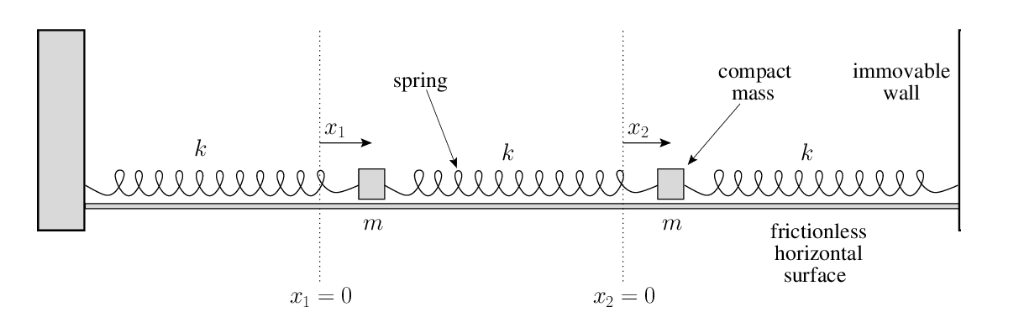
\includegraphics[scale=0.4]{figs/Coupled-Osc.png}
    \caption{}
    \label{fig:coupled-osc}
\end{figure}
\noindent
\textbf{(2)} Consider the mass-spring system as shown in the figure-\ref{fig:coupled-osc}


a. Show that, when written in terms of the physical coordinates, the total energy of the system 
takes the form,

\begin{equation*}
    E = m[\frac{1}{2}(\dot{x}_1^2+\dot{x}_2^2) + \omega_0^2(x_1^2-x_1 x_2+x_2^2)]
\end{equation*}

b. Furthermore, show that the total energy takes the form

\begin{equation*}
    E= m[(\dot{\eta}_1^2+\dot{\eta}_2^2) + \omega_0^2(\eta_1^2+3\eta_2^2)]
\end{equation*} 
when expressed in terms of the normal coordinates.

c. Hence, deduce that,

\hspace{2cm}
\begin{tabular}{l}
        (i) $E = m({\cal E}_1+{\cal E}_2)$\\
        (ii) ${\cal E}_1 = \dot{\eta}_{1}^{2} + \omega_{0}^{2} \eta_{1}^{2}$\\
        (iii) ${\cal E}_2 =\dot{\eta}_{2}^{2} + 3\omega_{0}^{2} \eta_{2}^{2}$\\
        (iv) $\frac{d{\cal E}_1}{dt}=0$\\
        (v) $\frac{d{\cal E}_2}{dt} =0$
\end{tabular}\\
Here, ${\cal E}_1$ and ${\cal E}_2$ are the separately conserved energies per unit masses of the 
first and second normal modes, respectively.\hfill \textbf{5+5+(4 + 2 + 2 + 1 + 1)}\\

\noindent

\section*{Part:B | Transverse Standing Waves \hfill \textbf{[15]}}

\textbf{(1)} Figure-\ref{fig:LC-chain} shows the left and right extremities of a linear LC 
network consisting of $N$ identical inductors of inductance $L$, and $N+1$ identical 
capacitors of capacitance $C$. Let the instantaneous current flowing through the $i$th 
inductor be $I_i(t)$, for $i=1,N$. Demonstrate from Kirchhoff's circuital laws that the 
currents evolve in time according to the coupled equations
\begin{equation*}
    \ddot{I}_i = \omega_{0}^{2} (I_{i-1} -2I_{i} + I_{i+1})
\end{equation*}
for $i=1,N$, where $\omega_0=1/\sqrt{LC}$, and $I_0=I_{N+1}=0$. Find the normal frequencies 
of the\\ system.\hfill \textbf{2+3}
\begin{figure}[h]
    \centering
    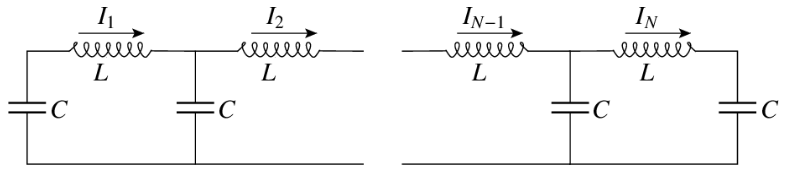
\includegraphics[scale=0.4]{figs/LC-chain.png}
    \caption{}
    \label{fig:LC-chain}
\end{figure}\\

\noindent
\textbf{(2)} The linear LC circuit considered in above question can be thought of as a discrete model 
of a uniform lossless transmission line (e.g., a co-axial cable). In this interpretation, $I_i(t)$ 
represents $I(x_i,t)$, where $x_i=i\delta x$. Moreover, $C={\cal C} \delta x$, and 
$L={\cal L} \delta x$, where ${\cal C}$ and ${\cal L}$ are the capacitance per unit length and 
the inductance per unit length of the line, respectively.

a. Show that, in the limit $\delta x\rightarrow 0$, the evolution equation for the coupled currents 
given in the above problem reduces to the wave equation,
\begin{equation*}
    \frac{\partial^2 I}{\partial t^2} = v^2 \frac{\partial^2 I}{\partial x^2}
\end{equation*}

b. If $V_i(t)$ is the potential difference (measured from the top to the bottom) across the $i+1$th 
capacitor (from the left) in the circuit shown in above problem, and $V(x,t)$ is the corresponding 
voltage in the transmission line, show that the discrete circuit equations relating the $I_i(t)$ 
and $V_i(t)$ reduce to
\begin{align*}
    \frac{\partial V}{\partial t}=-\frac{1}{{\cal C}}\frac{\partial I}{\partial x}\\
    \frac{\partial I}{\partial t}=-\frac{1}{{\cal L}}\frac{\partial V}{\partial x}
\end{align*}
in the transmission-line limit.

c. Demonstrate that the voltage in a transmission line satisfies the wave equation
\begin{equation*}
    \frac{\partial^2 V}{\partial t^2} = v^2\frac{\partial^2 V}{\partial x^2}.
\end{equation*}
\hfill \textbf{2 + (3 + 3) + 2}

\end{document}